\documentclass[12pt]{article}

\usepackage[a4paper,margin=2.5cm]{geometry}
\usepackage{amsmath, amssymb, amsthm}
\usepackage{bm}
\usepackage{hyperref}
\usepackage{graphicx}
\usepackage{caption}
\usepackage{listings}
\usepackage{xcolor}
\usepackage{float}
\usepackage{placeins}
\graphicspath{{figures/}}

\lstdefinestyle{code}{
  basicstyle=\ttfamily\small,
  numbers=left,
  numberstyle=\tiny,
  numbersep=8pt,
  keywordstyle=\color{blue},
  commentstyle=\color{teal!70!black},
  stringstyle=\color{orange!70!black},
  showstringspaces=false,
  breaklines=true,
  frame=single,
  framerule=0.3pt,
  rulecolor=\color{black!15}
}
\lstset{style=code}

\title{Independent Component Analysis Tutorial}
\author{}
\date{\today}

\begin{document}
\maketitle

\section{Introduction}
Independent Component Analysis (ICA) separates mixed signals into statistically independent sources using higher-order statistics. In contrast to PCA, which decorrelates by second-order moments, ICA seeks directions where components exhibit maximal non-Gaussianity, enabling blind source separation in audio, imaging, and biomedical data.

\section{Theory and Formulas}
\subsection{Linear Mixing Model}
Assume observed data \(\mathbf{x} = \mathbf{A}\mathbf{s}\), where \(\mathbf{s}\) contains independent sources with unit variance and \(\mathbf{A}\) is an invertible mixing matrix. ICA estimates an unmixing matrix \(\mathbf{W}\) so that \(\hat{\mathbf{s}} = \mathbf{W}\mathbf{x}\) approximates the original sources.

\subsection{Non-Gaussianity Maximization}
Many ICA algorithms maximize a contrast function \(J(\mathbf{w})\) measuring non-Gaussianity of projections. FastICA employs negentropy approximations with non-linearities such as \(g(u)=\tanh(u)\) or \(g(u)=u^3\):
\begin{equation}
\mathbf{w}_{\text{new}} = \mathbb{E}[\mathbf{x}g(\mathbf{w}^\top\mathbf{x})] - \mathbb{E}[g'(\mathbf{w}^\top\mathbf{x})]\mathbf{w}.
\end{equation}
Vectors are decorrelated after each update to enforce orthogonality across components.

\subsection{Whitening and Convergence}
Whitening the data (\(\mathbf{z}=\mathbf{V}^{-1/2}\mathbf{x}\)) simplifies estimation by ensuring uncorrelated unit-variance mixtures. Convergence is tracked via change in \(\mathbf{w}\) or the likelihood. Scale and permutation indeterminacies remain: components may be recovered up to sign and ordering.

\section{Applications and Tips}
\begin{itemize}
  \item \textbf{Blind source separation}: unmix audio recordings, EEG signals, or hyperspectral pixels.
  \item \textbf{Feature extraction}: provide statistically independent factors for downstream models.
  \item \textbf{Anomaly detection}: analyze independent components for sparse activations indicative of events.
  \item \textbf{Best practices}: center and whiten data, choose component counts carefully, and validate with reconstruction or domain knowledge.
\end{itemize}

\section{Python Practice}
The script \texttt{gen\_ica\_figures.py} creates synthetic source signals, mixes them, applies FastICA, and visualizes both the separated signals and the mixing/unmixing matrices.
\begin{lstlisting}[language=Python,caption={Excerpt from gen_ica_figures.py}]
from sklearn.decomposition import FastICA

ica = FastICA(n_components=3, whiten='unit-variance', random_state=0)
sources_hat = ica.fit_transform(mixed_signals)

mixing = ica.mixing_
unmixing = ica.components_
\end{lstlisting}

\section{Result}
\begin{figure}[H]
  \centering
  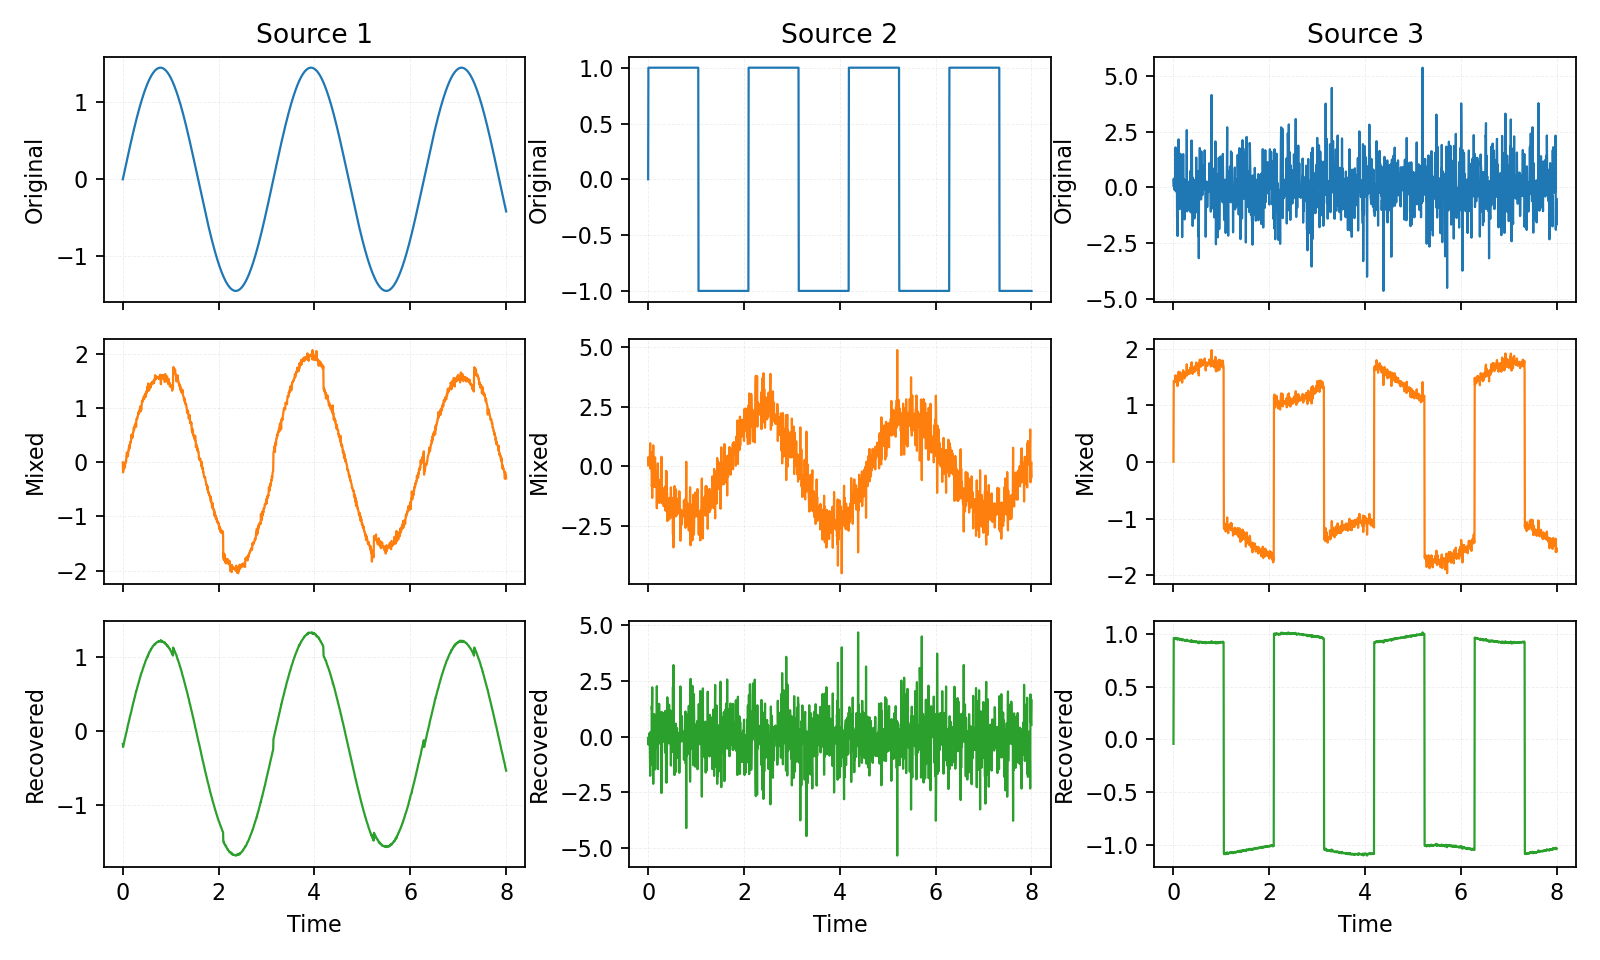
\includegraphics[width=0.85\linewidth]{ica_sources_vs_recovered.png}
  \caption{Comparison between original sources, mixed signals, and ICA-recovered components}
  \label{fig:ica_sources_vs_recovered}
\end{figure}

\begin{figure}[H]
  \centering
  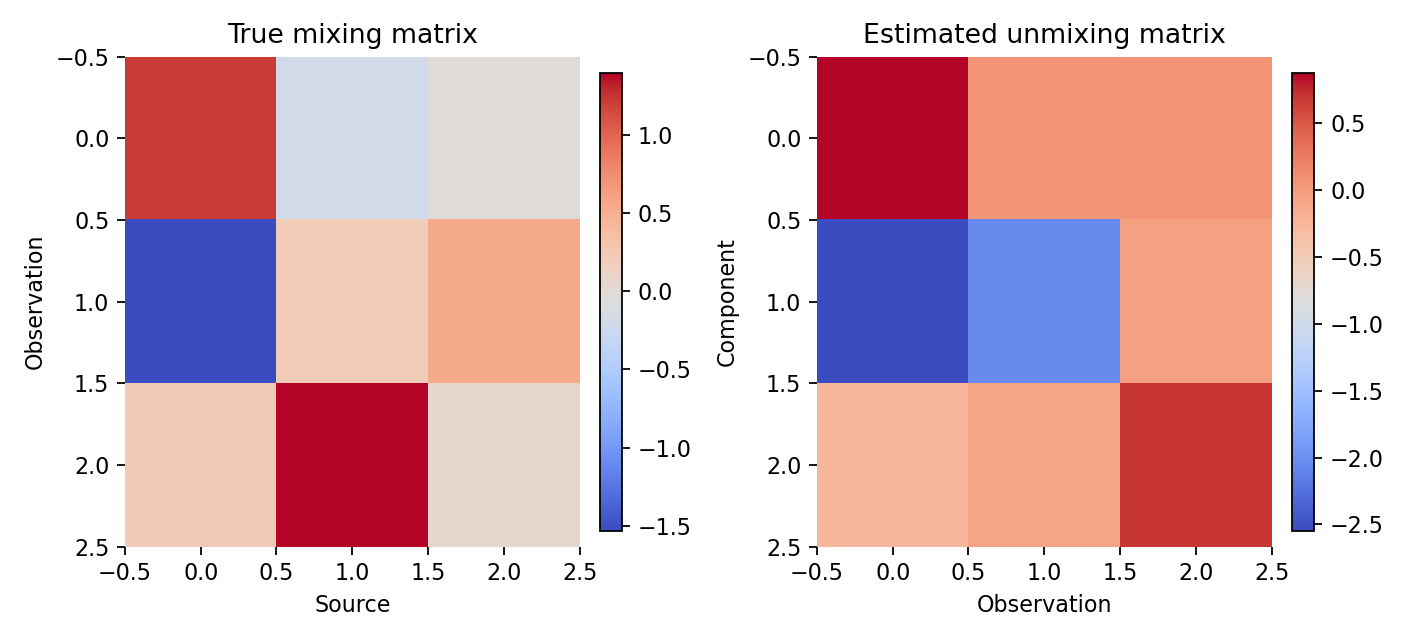
\includegraphics[width=0.75\linewidth]{ica_mixing_matrices.png}
  \caption{Heatmaps of true mixing matrix and estimated unmixing matrix}
  \label{fig:ica_mixing_matrices}
\end{figure}

\FloatBarrier
\section{Summary}
ICA goes beyond decorrelation by leveraging non-Gaussianity to recover latent sources. Whitening, iterative contrast optimization, and post-hoc validation are key to reliable separation. The example demonstrates how time-series visualizations and matrix comparisons help verify ICA performance.

\end{document}
